\begin{figure}[H]
	\centering
	\begin{tabular}{cc}
		\centering
		{\scriptsize 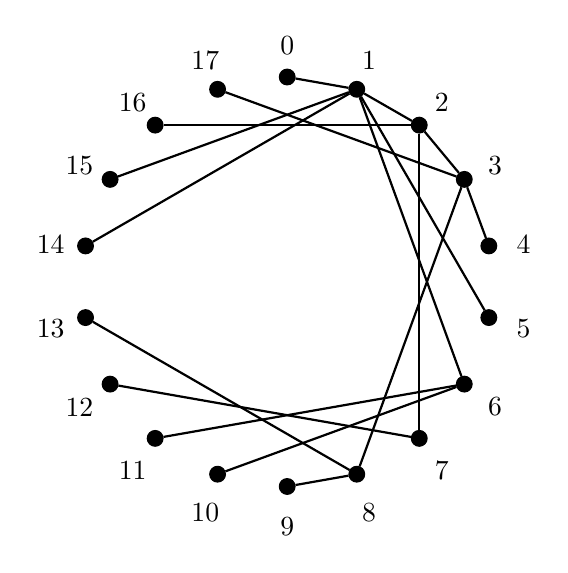
\begin{tikzpicture}
	\tikzset{enclosed/.style={draw, circle, inner sep=0pt, minimum size=0.2cm, fill=black}}

	\node[enclosed, label={above, xshift=0cm, yshift=0.052cm:0}] at (3.38, 5.2)(0){};
	\node[enclosed, label={above, xshift=0.156cm, yshift=0.026cm:1}] at (4.264, 5.044)(1){};
	\node[enclosed, label={above, xshift=0.286cm, yshift=-0.052cm:2}] at (5.057, 4.589)(2){};
	\node[enclosed, label={above, xshift=0.39cm, yshift=-0.169cm:3}] at (5.629, 3.9)(3){};
	\node[enclosed, label={above, xshift=0.442cm, yshift=-0.325cm:4}] at (5.941, 3.055)(4){};
	\node[enclosed, label={above, xshift=0.442cm, yshift=-0.481cm:5}] at (5.941, 2.145)(5){};
	\node[enclosed, label={above, xshift=0.39cm, yshift=-0.624cm:6}] at (5.629, 1.3)(6){};
	\node[enclosed, label={above, xshift=0.286cm, yshift=-0.754cm:7}] at (5.057, 0.611)(7){};
	\node[enclosed, label={above, xshift=0.156cm, yshift=-0.832cm:8}] at (4.264, 0.156)(8){};
	\node[enclosed, label={above, xshift=0cm, yshift=-0.858cm:9}] at (3.38, 0)(9){};
	\node[enclosed, label={above, xshift=-0.156cm, yshift=-0.832cm:10}] at (2.496, 0.156)(10){};
	\node[enclosed, label={above, xshift=-0.286cm, yshift=-0.754cm:11}] at (1.703, 0.611)(11){};
	\node[enclosed, label={above, xshift=-0.39cm, yshift=-0.637cm:12}] at (1.131, 1.3)(12){};
	\node[enclosed, label={above, xshift=-0.442cm, yshift=-0.481cm:13}] at (0.819, 2.145)(13){};
	\node[enclosed, label={above, xshift=-0.442cm, yshift=-0.325cm:14}] at (0.819, 3.055)(14){};
	\node[enclosed, label={above, xshift=-0.39cm, yshift=-0.169cm:15}] at (1.131, 3.9)(15){};
	\node[enclosed, label={above, xshift=-0.286cm, yshift=-0.052cm:16}] at (1.703, 4.589)(16){};
	\node[enclosed, label={above, xshift=-0.156cm, yshift=0.026cm:17}] at (2.496, 5.044)(17){};
	\draw [thick] (0)--(1);
	\draw [thick] (1)--(2);
	\draw [thick] (1)--(5);
	\draw [thick] (1)--(6);
	\draw [thick] (1)--(14);
	\draw [thick] (1)--(15);
	\draw [thick] (2)--(3);
	\draw [thick] (2)--(7);
	\draw [thick] (2)--(16);
	\draw [thick] (3)--(4);
	\draw [thick] (3)--(8);
	\draw [thick] (3)--(17);
	\draw [thick] (6)--(10);
	\draw [thick] (6)--(11);
	\draw [thick] (7)--(12);
	\draw [thick] (8)--(9);
	\draw [thick] (8)--(13);
\end{tikzpicture}

}&{\scriptsize 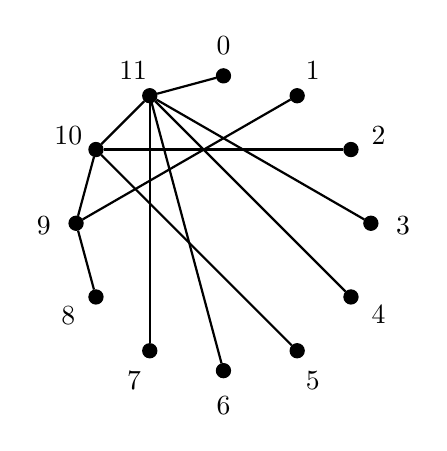
\begin{tikzpicture}[scale=0.8]
	\tikzset{enclosed/.style={draw, circle, inner sep=0pt, minimum size=0.18cm, fill=black}}

	\node[enclosed, label={above, xshift=0cm, yshift=0.0468cm:0}] at (3.042, 4.68)(0){};
	\node[enclosed, label={above, xshift=0.1989cm, yshift=-0.0117cm:1}] at (4.212, 4.3641)(1){};
	\node[enclosed, label={above, xshift=0.351cm, yshift=-0.1521cm:2}] at (5.0661, 3.51)(2){};
	\node[enclosed, label={above, xshift=0.4095cm, yshift=-0.3627cm:3}] at (5.382, 2.34)(3){};
	\node[enclosed, label={above, xshift=0.351cm, yshift=-0.5616cm:4}] at (5.0661, 1.17)(4){};
	\node[enclosed, label={above, xshift=0.1989cm, yshift=-0.7137cm:5}] at (4.212, 0.3159)(5){};
	\node[enclosed, label={above, xshift=0cm, yshift=-0.7722cm:6}] at (3.042, 0)(6){};
	\node[enclosed, label={above, xshift=-0.1989cm, yshift=-0.7137cm:7}] at (1.872, 0.3159)(7){};
	\node[enclosed, label={above, xshift=-0.351cm, yshift=-0.5733cm:8}] at (1.0179, 1.17)(8){};
	\node[enclosed, label={above, xshift=-0.4095cm, yshift=-0.3627cm:9}] at (0.702, 2.34)(9){};
	\node[enclosed, label={above, xshift=-0.351cm, yshift=-0.1521cm:10}] at (1.0179, 3.51)(10){};
	\node[enclosed, label={above, xshift=-0.2106cm, yshift=-0.0117cm:11}] at (1.872, 4.3641)(11){};
	\draw [thick] (0)--(11);
	\draw [thick] (9)--(1);
	\draw [thick] (9)--(8);
	\draw [thick] (10)--(2);
	\draw [thick] (10)--(5);
	\draw [thick] (10)--(9);
	\draw [thick] (11)--(3);
	\draw [thick] (11)--(4);
	\draw [thick] (11)--(6);
	\draw [thick] (11)--(7);
	\draw [thick] (11)--(10);
\end{tikzpicture}

}\\
		{\scriptsize 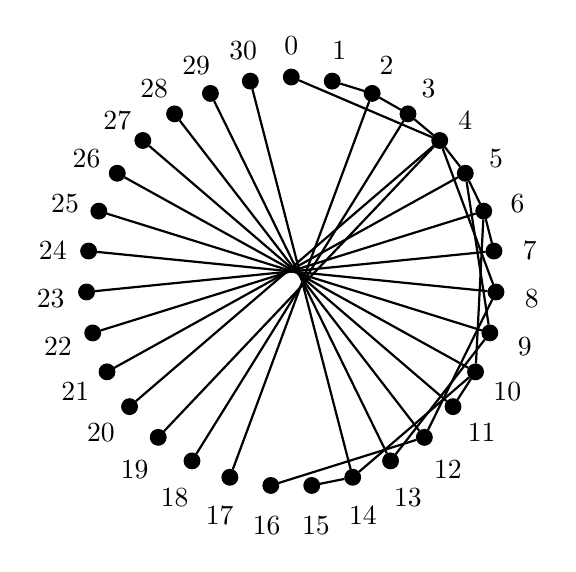
\begin{tikzpicture}
	\tikzset{enclosed/.style={draw, circle, inner sep=0pt, minimum size=0.2cm, fill=black}}

	\node[enclosed, label={above, xshift=0cm, yshift=0.052cm:0}] at (3.38, 5.2)(0){};
	\node[enclosed, label={above, xshift=0.091cm, yshift=0.039cm:1}] at (3.9, 5.148)(1){};
	\node[enclosed, label={above, xshift=0.182cm, yshift=0.013cm:2}] at (4.407, 4.992)(2){};
	\node[enclosed, label={above, xshift=0.26cm, yshift=-0.026cm:3}] at (4.862, 4.732)(3){};
	\node[enclosed, label={above, xshift=0.325cm, yshift=-0.091cm:4}] at (5.265, 4.394)(4){};
	\node[enclosed, label={above, xshift=0.39cm, yshift=-0.156cm:5}] at (5.59, 3.978)(5){};
	\node[enclosed, label={above, xshift=0.429cm, yshift=-0.247cm:6}] at (5.824, 3.497)(6){};
	\node[enclosed, label={above, xshift=0.455cm, yshift=-0.338cm:7}] at (5.954, 2.99)(7){};
	\node[enclosed, label={above, xshift=0.455cm, yshift=-0.429cm:8}] at (5.98, 2.47)(8){};
	\node[enclosed, label={above, xshift=0.442cm, yshift=-0.52cm:9}] at (5.902, 1.95)(9){};
	\node[enclosed, label={above, xshift=0.403cm, yshift=-0.598cm:10}] at (5.72, 1.456)(10){};
	\node[enclosed, label={above, xshift=0.364cm, yshift=-0.676cm:11}] at (5.434, 1.014)(11){};
	\node[enclosed, label={above, xshift=0.299cm, yshift=-0.754cm:12}] at (5.07, 0.624)(12){};
	\node[enclosed, label={above, xshift=0.221cm, yshift=-0.806cm:13}] at (4.641, 0.325)(13){};
	\node[enclosed, label={above, xshift=0.13cm, yshift=-0.832cm:14}] at (4.16, 0.117)(14){};
	\node[enclosed, label={above, xshift=0.052cm, yshift=-0.858cm:15}] at (3.64, 0.013)(15){};
	\node[enclosed, label={above, xshift=-0.052cm, yshift=-0.858cm:16}] at (3.12, 0.013)(16){};
	\node[enclosed, label={above, xshift=-0.13cm, yshift=-0.832cm:17}] at (2.6, 0.117)(17){};
	\node[enclosed, label={above, xshift=-0.221cm, yshift=-0.806cm:18}] at (2.119, 0.325)(18){};
	\node[enclosed, label={above, xshift=-0.299cm, yshift=-0.754cm:19}] at (1.69, 0.624)(19){};
	\node[enclosed, label={above, xshift=-0.364cm, yshift=-0.676cm:20}] at (1.326, 1.014)(20){};
	\node[enclosed, label={above, xshift=-0.403cm, yshift=-0.598cm:21}] at (1.04, 1.456)(21){};
	\node[enclosed, label={above, xshift=-0.442cm, yshift=-0.52cm:22}] at (0.858, 1.95)(22){};
	\node[enclosed, label={above, xshift=-0.455cm, yshift=-0.429cm:23}] at (0.78, 2.47)(23){};
	\node[enclosed, label={above, xshift=-0.455cm, yshift=-0.338cm:24}] at (0.806, 2.99)(24){};
	\node[enclosed, label={above, xshift=-0.429cm, yshift=-0.247cm:25}] at (0.936, 3.497)(25){};
	\node[enclosed, label={above, xshift=-0.39cm, yshift=-0.156cm:26}] at (1.17, 3.978)(26){};
	\node[enclosed, label={above, xshift=-0.325cm, yshift=-0.091cm:27}] at (1.495, 4.394)(27){};
	\node[enclosed, label={above, xshift=-0.26cm, yshift=-0.026cm:28}] at (1.898, 4.732)(28){};
	\node[enclosed, label={above, xshift=-0.182cm, yshift=0.013cm:29}] at (2.353, 4.992)(29){};
	\node[enclosed, label={above, xshift=-0.091cm, yshift=0.039cm:30}] at (2.86, 5.148)(30){};
	\draw [thick] (0)--(4);
	\draw [thick] (2)--(1);
	\draw [thick] (2)--(17);
	\draw [thick] (3)--(2);
	\draw [thick] (3)--(18);
	\draw [thick] (4)--(3);
	\draw [thick] (4)--(5);
	\draw [thick] (4)--(8);
	\draw [thick] (4)--(19);
	\draw [thick] (4)--(20);
	\draw [thick] (5)--(6);
	\draw [thick] (5)--(9);
	\draw [thick] (5)--(21);
	\draw [thick] (6)--(7);
	\draw [thick] (6)--(10);
	\draw [thick] (6)--(22);
	\draw [thick] (7)--(23);
	\draw [thick] (8)--(12);
	\draw [thick] (8)--(24);
	\draw [thick] (9)--(13);
	\draw [thick] (9)--(25);
	\draw [thick] (10)--(11);
	\draw [thick] (10)--(14);
	\draw [thick] (10)--(26);
	\draw [thick] (11)--(27);
	\draw [thick] (12)--(16);
	\draw [thick] (12)--(28);
	\draw [thick] (13)--(29);
	\draw [thick] (14)--(15);
	\draw [thick] (14)--(30);
\end{tikzpicture}

}&{\scriptsize 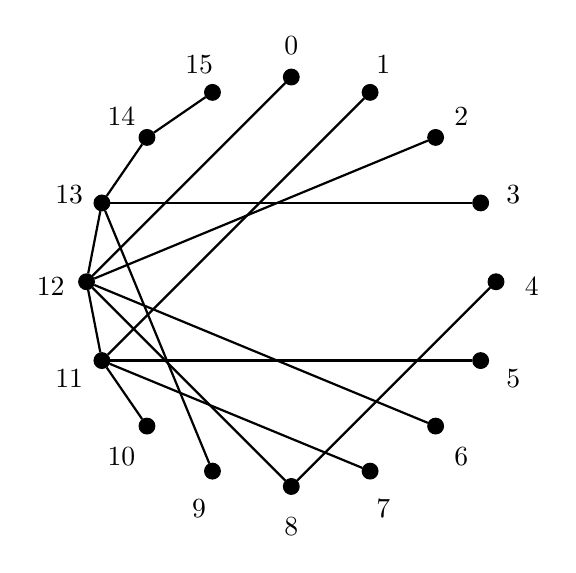
\begin{tikzpicture}
	\tikzset{enclosed/.style={draw, circle, inner sep=0pt, minimum size=0.2cm, fill=black}}

	\node[enclosed, label={above, xshift=0cm, yshift=0.052cm:0}] at (3.38, 5.2)(0){};
	\node[enclosed, label={above, xshift=0.169cm, yshift=0.013cm:1}] at (4.381, 5.005)(1){};
	\node[enclosed, label={above, xshift=0.325cm, yshift=-0.078cm:2}] at (5.213, 4.433)(2){};
	\node[enclosed, label={above, xshift=0.416cm, yshift=-0.234cm:3}] at (5.785, 3.601)(3){};
	\node[enclosed, label={above, xshift=0.455cm, yshift=-0.403cm:4}] at (5.98, 2.6)(4){};
	\node[enclosed, label={above, xshift=0.416cm, yshift=-0.572cm:5}] at (5.785, 1.599)(5){};
	\node[enclosed, label={above, xshift=0.325cm, yshift=-0.728cm:6}] at (5.213, 0.767)(6){};
	\node[enclosed, label={above, xshift=0.169cm, yshift=-0.819cm:7}] at (4.381, 0.195)(7){};
	\node[enclosed, label={above, xshift=0cm, yshift=-0.858cm:8}] at (3.38, 0)(8){};
	\node[enclosed, label={above, xshift=-0.169cm, yshift=-0.819cm:9}] at (2.379, 0.195)(9){};
	\node[enclosed, label={above, xshift=-0.325cm, yshift=-0.728cm:10}] at (1.547, 0.767)(10){};
	\node[enclosed, label={above, xshift=-0.416cm, yshift=-0.572cm:11}] at (0.975, 1.599)(11){};
	\node[enclosed, label={above, xshift=-0.455cm, yshift=-0.403cm:12}] at (0.78, 2.6)(12){};
	\node[enclosed, label={above, xshift=-0.416cm, yshift=-0.234cm:13}] at (0.975, 3.601)(13){};
	\node[enclosed, label={above, xshift=-0.325cm, yshift=-0.078cm:14}] at (1.547, 4.433)(14){};
	\node[enclosed, label={above, xshift=-0.169cm, yshift=0.013cm:15}] at (2.379, 5.005)(15){};
	\draw [thick] (0)--(12);
	\draw [thick] (8)--(4);
	\draw [thick] (11)--(1);
	\draw [thick] (11)--(5);
	\draw [thick] (11)--(7);
	\draw [thick] (11)--(10);
	\draw [thick] (12)--(2);
	\draw [thick] (12)--(6);
	\draw [thick] (12)--(8);
	\draw [thick] (12)--(11);
	\draw [thick] (12)--(13);
	\draw [thick] (13)--(3);
	\draw [thick] (13)--(9);
	\draw [thick] (13)--(14);
	\draw [thick] (14)--(15);
\end{tikzpicture}

}\\
		{\scriptsize 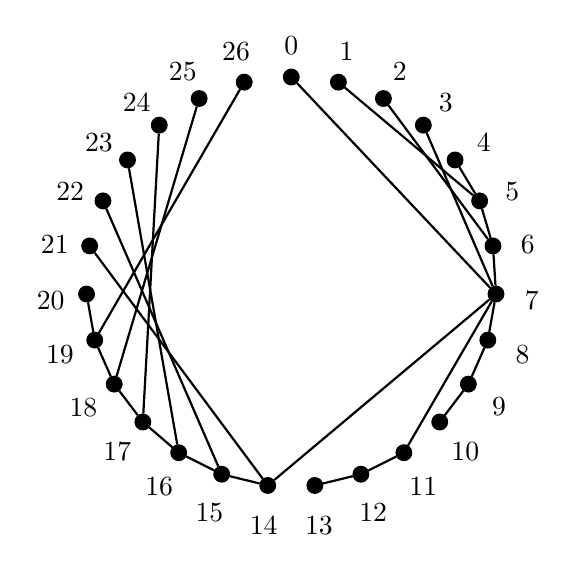
\begin{tikzpicture}
	\tikzset{enclosed/.style={draw, circle, inner sep=0pt, minimum size=0.2cm, fill=black}}

	\node[enclosed, label={above, xshift=0cm, yshift=0.052cm:0}] at (3.38, 5.2)(0){};
	\node[enclosed, label={above, xshift=0.104cm, yshift=0.039cm:1}] at (3.978, 5.135)(1){};
	\node[enclosed, label={above, xshift=0.208cm, yshift=0cm:2}] at (4.55, 4.927)(2){};
	\node[enclosed, label={above, xshift=0.286cm, yshift=-0.052cm:3}] at (5.057, 4.589)(3){};
	\node[enclosed, label={above, xshift=0.364cm, yshift=-0.13cm:4}] at (5.46, 4.147)(4){};
	\node[enclosed, label={above, xshift=0.416cm, yshift=-0.221cm:5}] at (5.772, 3.627)(5){};
	\node[enclosed, label={above, xshift=0.442cm, yshift=-0.325cm:6}] at (5.941, 3.055)(6){};
	\node[enclosed, label={above, xshift=0.455cm, yshift=-0.429cm:7}] at (5.98, 2.444)(7){};
	\node[enclosed, label={above, xshift=0.442cm, yshift=-0.533cm:8}] at (5.876, 1.859)(8){};
	\node[enclosed, label={above, xshift=0.39cm, yshift=-0.624cm:9}] at (5.629, 1.3)(9){};
	\node[enclosed, label={above, xshift=0.325cm, yshift=-0.715cm:10}] at (5.265, 0.819)(10){};
	\node[enclosed, label={above, xshift=0.247cm, yshift=-0.78cm:11}] at (4.81, 0.429)(11){};
	\node[enclosed, label={above, xshift=0.156cm, yshift=-0.832cm:12}] at (4.264, 0.156)(12){};
	\node[enclosed, label={above, xshift=0.052cm, yshift=-0.858cm:13}] at (3.679, 0.013)(13){};
	\node[enclosed, label={above, xshift=-0.052cm, yshift=-0.858cm:14}] at (3.081, 0.013)(14){};
	\node[enclosed, label={above, xshift=-0.156cm, yshift=-0.832cm:15}] at (2.496, 0.156)(15){};
	\node[enclosed, label={above, xshift=-0.247cm, yshift=-0.78cm:16}] at (1.95, 0.429)(16){};
	\node[enclosed, label={above, xshift=-0.325cm, yshift=-0.715cm:17}] at (1.495, 0.819)(17){};
	\node[enclosed, label={above, xshift=-0.39cm, yshift=-0.637cm:18}] at (1.131, 1.3)(18){};
	\node[enclosed, label={above, xshift=-0.442cm, yshift=-0.533cm:19}] at (0.884, 1.859)(19){};
	\node[enclosed, label={above, xshift=-0.455cm, yshift=-0.429cm:20}] at (0.78, 2.444)(20){};
	\node[enclosed, label={above, xshift=-0.442cm, yshift=-0.325cm:21}] at (0.819, 3.055)(21){};
	\node[enclosed, label={above, xshift=-0.416cm, yshift=-0.221cm:22}] at (0.988, 3.627)(22){};
	\node[enclosed, label={above, xshift=-0.364cm, yshift=-0.13cm:23}] at (1.3, 4.147)(23){};
	\node[enclosed, label={above, xshift=-0.286cm, yshift=-0.052cm:24}] at (1.703, 4.589)(24){};
	\node[enclosed, label={above, xshift=-0.208cm, yshift=0cm:25}] at (2.21, 4.927)(25){};
	\node[enclosed, label={above, xshift=-0.104cm, yshift=0.039cm:26}] at (2.782, 5.135)(26){};
	\draw [thick] (0)--(7);
	\draw [thick] (5)--(1);
	\draw [thick] (5)--(4);
	\draw [thick] (6)--(2);
	\draw [thick] (6)--(5);
	\draw [thick] (7)--(3);
	\draw [thick] (7)--(6);
	\draw [thick] (7)--(8);
	\draw [thick] (7)--(11);
	\draw [thick] (7)--(14);
	\draw [thick] (8)--(9);
	\draw [thick] (9)--(10);
	\draw [thick] (11)--(12);
	\draw [thick] (12)--(13);
	\draw [thick] (14)--(15);
	\draw [thick] (14)--(21);
	\draw [thick] (15)--(16);
	\draw [thick] (15)--(22);
	\draw [thick] (16)--(17);
	\draw [thick] (16)--(23);
	\draw [thick] (17)--(18);
	\draw [thick] (17)--(24);
	\draw [thick] (18)--(19);
	\draw [thick] (18)--(25);
	\draw [thick] (19)--(20);
	\draw [thick] (19)--(26);
\end{tikzpicture}

}&{\scriptsize 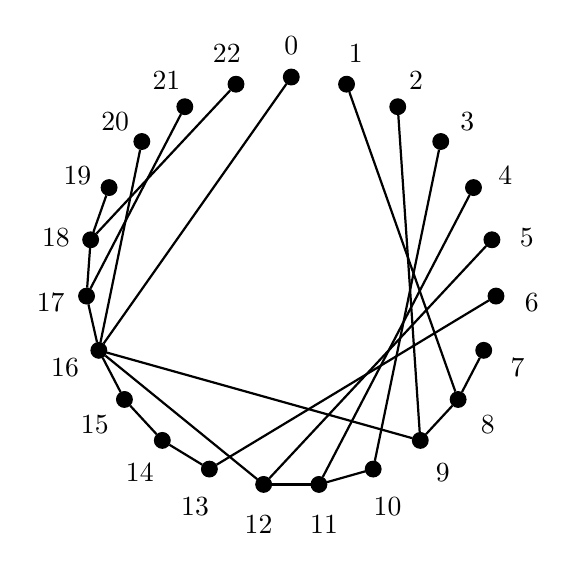
\begin{tikzpicture}
	\tikzset{enclosed/.style={draw, circle, inner sep=0pt, minimum size=0.2cm, fill=black}}

	\node[enclosed, label={above, xshift=0cm, yshift=0.052cm:0}] at (3.38, 5.2)(0){};
	\node[enclosed, label={above, xshift=0.117cm, yshift=0.039cm:1}] at (4.082, 5.109)(1){};
	\node[enclosed, label={above, xshift=0.234cm, yshift=-0.013cm:2}] at (4.732, 4.823)(2){};
	\node[enclosed, label={above, xshift=0.338cm, yshift=-0.091cm:3}] at (5.278, 4.381)(3){};
	\node[enclosed, label={above, xshift=0.403cm, yshift=-0.195cm:4}] at (5.694, 3.796)(4){};
	\node[enclosed, label={above, xshift=0.442cm, yshift=-0.312cm:5}] at (5.928, 3.133)(5){};
	\node[enclosed, label={above, xshift=0.455cm, yshift=-0.429cm:6}] at (5.98, 2.418)(6){};
	\node[enclosed, label={above, xshift=0.429cm, yshift=-0.559cm:7}] at (5.824, 1.729)(7){};
	\node[enclosed, label={above, xshift=0.377cm, yshift=-0.663cm:8}] at (5.499, 1.105)(8){};
	\node[enclosed, label={above, xshift=0.286cm, yshift=-0.754cm:9}] at (5.018, 0.585)(9){};
	\node[enclosed, label={above, xshift=0.182cm, yshift=-0.819cm:10}] at (4.42, 0.221)(10){};
	\node[enclosed, label={above, xshift=0.065cm, yshift=-0.858cm:11}] at (3.731, 0.026)(11){};
	\node[enclosed, label={above, xshift=-0.065cm, yshift=-0.858cm:12}] at (3.029, 0.026)(12){};
	\node[enclosed, label={above, xshift=-0.182cm, yshift=-0.819cm:13}] at (2.34, 0.221)(13){};
	\node[enclosed, label={above, xshift=-0.286cm, yshift=-0.754cm:14}] at (1.742, 0.585)(14){};
	\node[enclosed, label={above, xshift=-0.377cm, yshift=-0.663cm:15}] at (1.261, 1.105)(15){};
	\node[enclosed, label={above, xshift=-0.429cm, yshift=-0.559cm:16}] at (0.936, 1.729)(16){};
	\node[enclosed, label={above, xshift=-0.455cm, yshift=-0.429cm:17}] at (0.78, 2.418)(17){};
	\node[enclosed, label={above, xshift=-0.442cm, yshift=-0.312cm:18}] at (0.832, 3.133)(18){};
	\node[enclosed, label={above, xshift=-0.403cm, yshift=-0.195cm:19}] at (1.066, 3.796)(19){};
	\node[enclosed, label={above, xshift=-0.338cm, yshift=-0.091cm:20}] at (1.482, 4.381)(20){};
	\node[enclosed, label={above, xshift=-0.234cm, yshift=-0.013cm:21}] at (2.028, 4.823)(21){};
	\node[enclosed, label={above, xshift=-0.117cm, yshift=0.039cm:22}] at (2.678, 5.109)(22){};
	\draw [thick] (0)--(16);
	\draw [thick] (8)--(1);
	\draw [thick] (8)--(7);
	\draw [thick] (9)--(2);
	\draw [thick] (9)--(8);
	\draw [thick] (10)--(3);
	\draw [thick] (11)--(4);
	\draw [thick] (11)--(10);
	\draw [thick] (12)--(5);
	\draw [thick] (12)--(11);
	\draw [thick] (13)--(6);
	\draw [thick] (14)--(13);
	\draw [thick] (15)--(14);
	\draw [thick] (16)--(9);
	\draw [thick] (16)--(12);
	\draw [thick] (16)--(15);
	\draw [thick] (16)--(17);
	\draw [thick] (16)--(20);
	\draw [thick] (17)--(18);
	\draw [thick] (17)--(21);
	\draw [thick] (18)--(19);
	\draw [thick] (18)--(22);
\end{tikzpicture}

}\\
	\end{tabular}
	\caption{$CR(12, 4, 6)$の6つの独立全域木}
	\label{fig:CR(12, 4, 6)}
\end{figure}
